\section{Среда программирования роботов QReal:Robots}
\label{chapter:qRealRobots}
Наиболее зрелый на данный момент пример применения технологии QReal --- среда для 
обучения программированию в школах QReal:Robots. Этот проект создавался в практически 
идеальных для применения предметно-ориентированного подхода условиях: имелась достаточно 
узкая предметная область, в которой уже довольно активно применялось визуальное программирование, 
имелась потребность в средствах программирования в рамках этой предметной области для 
написания нетривиальных программ, имелась DSM-платформа QReal, на которой было возможно 
в короткие сроки реализовать такое решение. В этой работе результаты проекта QReal:Robots изложены достаточно кратко, более подробно см. статьи
\cite{bryksin2011robots, tikhonova2012robots, litvinov2012robots, terekhov2013robots}
%TODO Больше ссылок
Далее описание результатов приводится в такой последовательности --- приводится введение 
в предметную область и мотивация к созданию DSM-решения, анализ и формулировка требований, 
изложение возможностей визуального языка и инструментальных средств для него с точки 
зрения пользователя и "`ручной"' реализации, далее рассказывается, как при реализации 
DSM-решения применялись возможности платформы QReal, в чём она смогла помочь, а в чём нет, и почему.

\subsection{Постановка задачи}
Сейчас в школах для начального преподавания информатики активно внедряются робототехнические 
конструкторы, наиболее популярный из которых на данный момент --- конструктор LEGO Mindstorms NXT 2.0%
\footnote{Домашняя страница конструктора Mindstorms, URL: http://mindstorms.lego.com/ (дата обращения 07.09.2014)}%
. Идея использовать роботы для преподавания не случайна, понятие "`исполнитель"' традиционно 
используется в школьном преподавании в России со времён академика Ершова, а робот --- наиболее 
наглядный вид исполнителя. Исполнитель --- это некая сущность, способная выполнять 
команды, указанные в программе, в некоторой среде. До сих пор самым популярным исполнителем 
в школах остаётся "`черепашка"' LOGO%
\footnote{MyRobot, Язык программирования Лого, URL: http://myrobot.ru/logo/aboutlogo.php (дата обращения 07.09.2014)}%
, предложенная американским педагогом Сеймуром Пейпертом ещё в 1967 году. "`Черепашка"' 
может перемещаться по экрану, оставляя за собой след, и подчиняется командам вида "`поднять перо"', 
"`опустить перо"', "`20 шагов вперёд"', "`на 90 градусов налево"'. В текстовых программах 
может быть не очевидно, где исполнение алгоритма пошло не так, а иногда непонятно 
даже, правильно работает программа или нет. В случае с "`черепашкой"' отклонение выполнения 
программы от задумки автора будет видимо сразу же, "`черепашка"' нарисует что-то некорректное. 
При этом сразу видно, где допущена ошибка, можно легко найти строку программы, на 
которой "`черепашка"' отклонилась от задуманной траектории.

Исполнитель, движущийся по экрану, всё же оказывается недостаточно нагляден. Сеймур Пейперт 
в своих ранних экспериментах использовал механическую черепашку. Сейчас развитие электроники 
сделало возможным создавать относительно недорогие устройства, исполняющие программу 
с помощью дистанционного управления с компьютера или позволяющие загружать программу 
для автономного исполнения. Для преподавания в школах из таких устройств наиболее 
интересны робототехнические конструкторы, потому что они требуют сборки робота перед 
его программированием, что интереснее для детей и развивает их конструкторские навыки. 
Самый известный такой конструктор --- Mindstorms NXT. Он позволяет из трёх моторов, 
трёх видов датчиков (датчика касания, ультразвукового датчика расстояния, датчика 
освещённости), блока управления и пластмассовых деталей собирать довольно сложные 
конструкции, от движущихся тележек до стационарных устройств, например, для росписи 
ёлочных украшений или игры на барабанах. 

Программировать такие роботы сложнее, чем "`черепашку"', поскольку из конструктора 
можно собрать самые разные модели роботов, и программировать приходится в терминах, 
например, вида "`мотор А включить на 50\% мощности"', "`ждать срабатывания датчика касания"', 
а не "`вперёд на 20 шагов"', как в "`черепашке"'. Это интереснее и полезнее для детей, 
но сложнее. Дополнительную сложность добавляет и то, что робот может взаимодействовать 
с окружением с помощью датчиков, в отличие от "`черепашки"'. Это позволяет преподавать 
не только основы информатики, но и основы кибернетики, демонстрируя принципы построения 
программ, работающих во внешней среде, которую они не могут контролировать. Типичный 
пример задачи, которую решают начинающие программисты с помощью робота --- движение по линии, 
когда робот с одним или двумя датчиками освещённости должен проехать по чёрной линии, 
нарисованной на полу. На "`черепашке"' обучать решению подобных задач невозможно.

Сложность программирования робототехнических конструкторов преодолевается использованием 
визуальных языков программирования. Они гораздо понятнее и нагляднее для школьников, 
чем текстовые языки. Программы на таких языках состоят из элементарных блоков, например, 
"`включить мотор"', "`ждать срабатывания датчика"', которые достаточно перетащить с 
палитры на диаграмму и соединить связями. При наличии удобного редактора для такого 
языка пользоваться им могут даже дошкольники, не умеющие ещё читать. Как правило, с 
помощью визуальных языков школьники программируют примерно до седьмого класса, после 
чего постепенно переходят на текстовые языки. В комплекте с конструктором поставляется среда визуального программирования NXT-G
%TODO: Ссылка
, существуют отдельно распространяемые среды, самой популярной из которых в школах является Robolab~\cite{portsmore1999robolab}. 
Визуальное программирование в сообществе людей, занимающихся программированием таких роботов, весьма популярно.

Существующие среды программирования роботов имеют ряд недостатков, затрудняющих их 
использование в школах, например, отсутствие русификации, невозможность отладки программы. 
Это делает актуальной задачу создания новой такой среды, учитывающей все достоинства и 
недостатки существующих, а также уже накопленный опыт преподавания. Поэтому возникла 
ситуация, чрезвычайно интересная для апробации DSM---платформы. В выбранной предметной 
области уже сложились традиции использования визуальных языков, поэтому можно рассчитывать 
на содержательное сравнение с существующими средами. Кроме того, задачи, решаемые в 
данной предметной области, достаточно нетривиальны, чтобы полученный опыт разработки 
визуального языка можно было перенести на более сложные случаи, возникающие при промышленном 
программировании. Все типичные для императивного программирования конструкции, такие 
как ветвления и циклы, используются при программировании роботов, поэтому полученные 
результаты окажутся применимыми и для других случаев, где требуется императивный подход. 
Вместе с тем, предметная область достаточно узка, чтобы можно было получить заметные 
выгоды от использования предметно-ориентированного языка: на языке общего назначения программирование велось бы путём вызова функций API
\footnote{Application Program Interface, интерфейс прикладных программ}
 робота, для чего требовалось бы писать довольно много вспомогательного кода, например, объявления функций. Кроме того,
 при использовании визуального языка невозможно совершить некоторые ошибки, типичные 
для текстовых языков, например, невозможно ошибиться в написании имени вызываемой 
функции, если достаточно просто перетащить соответствующий ей блок из палитры.

\subsection{Существующие среды визуального программирования роботов}
Как уже отмечалось, визуальное программирование весьма популярно среди людей, работающих 
с конструкторами Mindstorms. Анализ существующих сред является естественным источником 
для формулировки требований к проектируемому DSM-решению, наряду с интервьюированием 
экспертов в предметной области и потенциальных пользователей. Результаты анализа 
существующих сред представлены ниже.

Среда NXT-G 
%TODO: Ссылка
поставляется вместе с конструктором Mindstorms NXT. Среда базируется на системе визуального программирования LabView
%TODO: Ссылка
, используемой для моделирования различных экспериментов. Среда LabView в качестве 
языка программирования использует визуальный язык G, язык с процессом вычислений, 
ориентированным на данные --- в нём связи между блоками обозначают не последовательность 
выполнения операторов, а зависимости между блоками по данным. Основная проблема среды NXT-G 
заключается в отсутствии полноценной поддержки математических выражений. В языке присутствуют 
блоки для арифметических действий, констант, переменных, и чтобы построить математическое
выражение, их надо соединять связями. Таким образом, на диаграмме приходится рисовать 
фактически дерево разбора арифметического выражения, что делает программирование даже 
несложных задач, требующих математики, чрезвычайно утомительным. В школьной программе 
такие задачи возникают часто, например, движение по линии или езда вдоль стены с помощью 
датчика расстояния требует вычисления производной, поэтому NXT-G для преподавания в 
школах практически не используется. Ещё одной особенностью этой среды, оказавшейся 
недостатком при преподавании в школах, стало то, что не все свойства блоков видны 
на диаграмме, требуется кликнуть на блок и открыть его свойства в редакторе свойств. 
Это делает невозможным показ всей программы на проекторе, что затрудняет воспроизведение 
программы учениками. У NXT-G нет официальной русификации, отсутствуют встроенные 
средства отладки и генерации текстовой формы языка. Возможно добавление сторонних 
блоков средствами LabView, сам NXT-G позволяет выделять фрагменты диаграмм в подпрограммы 
и использовать их с помощью специального блока.

Среда Robolab
%TODO: Ссылка
также создавалась на основе среды LabView, и, в отличие от NXT-G, создавалась 
специально для преподавания. Примером специфичного для преподавания решения, принятого 
в среде Robolab, может послужить разделение возможностей среды на уровни. При запуске 
среды предлагается выбрать уровень, на котором будет вестись работа, на первых уровнях 
пользователь может только заполнять пустые места в уже готовом шаблоне программы, 
используя очень ограниченный набор блоков. На более высоких уровнях предоставляется 
возможность самостоятельно задавать связи между блоками, доступно больше различных 
видов блоков (например, на начальном уровне есть блок "`ждать"', на более высоком --- 
набор блоков "`ждать 1 сек"', "`ждать 2 сек"', "`ждать 5 сек"' и т.д., на ещё более 
высоком --- "`ждать N сек"', где N является параметром блока и может являться результатом 
вычисления. Такое разделение позволяет начать работу со средой детям дошкольного возраста, 
которые не умеют ещё даже читать (картинки, используемые в блоках, достаточно понятны), 
при этом дети могут исследовать среду и разбираться в функциональности более высоких 
уровней постепенно, практически без помощи преподавателей.

Математические выражения Robolab поддерживает гораздо лучше, чем NXT-G, позволяя писать 
произвольные выражения в виде текста, используя тригонометрические функции и переменные, 
обращаться к значениям, возвращаемым датчиками, прямо из выражений. Циклы в Robolab 
реализованы довольно необычно --- есть блоки "`начало цикла"' и "`конец цикла"', связь 
между концом и началом никак не визуализируется. Есть довольно развитая поддержка 
параллельных задач, есть все необходимые конструкции императивного программирования, 
включая подпрограммы. Русифицирована среда лишь частично, не имеет встроенных средств 
отладки, не может порождать код программы в текстовом виде, имеет довольно несовременный 
пользовательский интерфейс, при этом не бесплатна, и стоит довольно дорого для российских 
школ. При этом, несмотря на все перечисленные недостатки, эта среда вполне подходит 
для иллюстрации материала информатики и кибернетики примерно до 7-го класса школы,
и сейчас является самой распространённой в школах России.

Среда Microsoft Robotics Developer Studio (MRDS)
%TODO: Ссылка
, в отличие от рассмотренных ранее сред, не создавалась исключительно для конструктора 
Mindstorms NXT. Среда предназначена для создания сложных многопоточных приложений с 
реактивной моделью поведения, которые весьма типичны для задач робототехники --- современная 
робототехническая система представляет собой целый комплекс вычислительных средств, 
часть из которых может быть установлена на роботе, а часть --- на компьютере, связанном 
с роботом скоростной сетью. Кроме того, необходимость в высокопроизводительных распределённых 
программных системах возникает не только в робототехнике, поэтому среда MRDS применяется 
и в других областях, например, с её помощью разрабатывались серверные части крупных веб-приложений
%TODO: ссылка на CCR at MySpace
. Программа в MRDS представляется в виде набора веб-сервисов, исполняемых независимо 
и обменивающихся данными друг с другом. Процесс программирования сводится к связыванию 
входов и выходов предопределённых сервисов, что осуществляется на визуальном языке 
VPL (Visual Programming Language)
%TODO: Ссылка
. Этот язык, таким образом, попадает в категорию языков с процессом управления, ориентированным 
на данные, чем очень похож на визуальные языки систем, рассмотренных выше. Среда имеет 
развитую трехмерную среду симуляции, позволяя исполнять созданные программы не только 
на реальном роботе, но и на трёхмерной модели в окружении с подробной симуляцией физики 
(например, в стандартной поставке имеется подробная трёхмерная модель квартиры, по которой 
может перемещаться робот). Среда поддерживает генерацию кода на языке C\#, отладку, 
распространяется бесплатно.

Несмотря на всё это, среда MRDS очень редко используется в школах для преподавания 
информатики. Связано это прежде всего с используемой там моделью вычислений. Представлять 
программу в виде взаимодействующих независимо исполняющихся веб-сервисов удобно профессиональным 
программистам, но школьникам, впервые пробующим программировать, потребуется знать и 
уметь слишком многое, чтобы писать содержательные программы. К тому же, такой подход к 
программированию слишком специфичен и не может быть использован в качестве иллюстративного 
материала для "`обычного"' императивного программирования, знание которого будет необходимо 
школьникам в дальнейшем. Кроме того, генерируемый средой код не может быть исполнен 
непосредственно на роботе Mindstorms NXT --- он имеет слишком мало ресурсов для этого, 
робот может управляться только дистанционно по интерфейсу Bluetooth. Среда MRDS ориентирована 
на более дорогие устройства, в частности, "`стандартная модель"' робота, рекомендуемая 
для использования в MRDS включает в себя ноутбук в качестве блока управления, который 
один дороже всего конструктора Mindstorms NXT. Использование модели робота позволяет 
решить эту проблему только частично --- модель, даже с детальной реализацией физических 
эффектов, не позволяет воспроизвести всё многообразие реального мира, из-за которого, 
собственно, и возникают проблемы, которые решаются в кибернетике.

\subsection{Требования к DSM-решению}
По результатам анализа существующих сред и общения с экспертами предметной области 
(преподавателями и методистами, использующими робототехнические конструкторы в своей работе) 
были сформированы следующие требования к проектируемому DSM-решению.

\begin{enumerate}
	\item Среда должна позволять создавать довольно сложные программы, поскольку предполагается, 
		что она будет служить для иллюстрации нетривиальных вопросов информатики и кибернетики, 
		при этом её язык должен оставаться близким к "`традиционным"' императивным языкам 
		программирования. Среда должна удобно поддерживать нетривиальные математические 
		выражения, переменные, ветвления, циклы, параллельные задачи.
	\item Среда должна быть проста и удобна в работе, поскольку неудобный пользовательский 
		интерфейс создавал бы дополнительную когнитивную нагрузку при изучении и без того 
		сложного материала. Среда должна быть интуитивно понятна, работа со средой должна 
		быть возможна при минимальном участии преподавателя.
	\item Требуется наличие встроенных средств отладки, поскольку школьникам важно не 
		столько сделать работающую программу, сколько разобраться в том, как она работает. 
		Ошибки могут иметь большую педагогическую ценность, и среда должна иметь возможность 
		демонстрировать ошибки (и ход выполнения программы вообще) школьникам. Весьма желательна 
		возможность исполнения программы на модели робота на компьютере.
	\item Требуется наличие возможности порождения текстового представления программы. 
		Школьники старших классов, серьёзно занимающиеся программированием, должны видеть 
		связь между диаграммами и кодом на текстовых языках, иметь возможность редактировать 
		текстовую программу в той же среде, в которой они привыкли работать.
	\item Среда должна быть русскоязычной, поскольку основная группа её пользователей 
		ещё не владеет в должной степени иностранными языками.
\end{enumerate}

Как видно из приведённого выше обзора, ни одна из существующих сред программирования 
роботов указанным требованиям не удовлетворяет. Наиболее активно в школах используется 
среда Robolab, но, поскольку он недёшев, среди школьных учителей есть желание заменить 
её на более современный (и по возможности бесплатный) аналог. Поэтому существует реальная 
потребность в создании новой такой среды, что и было сделано на базе метатехнологии QReal.

\subsection{Визуальный язык QReal:Robots}
В качестве модели вычислений для визуального языка в силу наличия требования близости 
к "`традиционным"' языкам программирования была выбрана модель вычислений, ориентированная 
на поток исполнения. Блок языка представляет собой элементарную команду роботу, связи 
между блоками указывают последовательность, в которой выполняются блоки, это делает 
программы больше похожими на блок-схемы, чем программы на существующих средах программирования 
роботов. Пример программы приведён на рисунке~\ref{image:robotsProgramExample}. Двухмоторная 
тележка с датчиком касания под управлением этой программы будет двигаться до срабатывания 
датчика касания, после чего подаст звуковой сигнал и будет некоторое время двигаться 
в обратном направлении, после чего повторит действия сначала.

\begin{figure} [ht]
	\begin{center}
		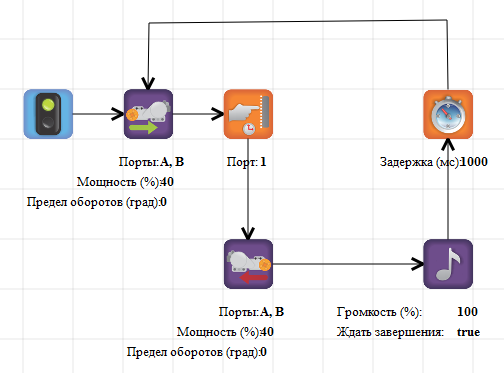
\includegraphics[width=0.6\textwidth]{part5/5.1/robotsProgramExample.png}
		\caption{Пример программы QReal:Robots.}
		\label{image:robotsProgramExample}
	\end{center}
\end{figure}

Все блоки языка разбиты на смысловые группы, которые могут быть отдельно свёрнуты 
или развёрнуты в палитре. Описание для каждого блока приведено ниже.

%TODO: Таблица?
%TODO: Обновить описание
\begin{enumerate}
	\item Группа "`Алгоритмы"' предназначена для блоков, определяющих последовательность 
		выполнения команд программы.
		\begin{enumerate}
			\item "`Диаграмма поведения робота"' --- блок, на который добавляются все остальные 
				блоки программы. Обычно непосредственно в рабочей области не рисуется, но 
				при создании новой диаграммы перетаскивается из палитры в обозреватель модели.
			\item "`Линия соединения"' --- единственная связь, присутствующая в языке, задаёт 
				последовательность исполнения блоков. Имеет метку, которая позволяет определять, 
				когда управление надо передать по линии соединения в случае условного оператора 
				или цикла --- например, метка "`больше 0"' говорит, что управление по данной 
				связи будет передано только тогда, когда выражение в условном операторе, подключённом 
				к этой связи, будет иметь значение, большее 0. По умолчанию связи не помечены ничем.
			\item "`Условие"' --- условный оператор. Параметризуется арифметическим выражением 
				и должен иметь две исходящие связи, одна из которых выбирается для передачи 
				управления в зависимости от значения выражения и метки связи.
			\item "`Цикл"' --- оператор цикла, параметризуется арифметическим выражением, 
				значение которого будет количеством итераций, которые надо выполнить, и должен 
				иметь две исходящие связи. Пока блок посещён меньшее количество раз, чем желаемое 
				количество итераций, управление передаётся по связи, помеченной как "`итерация"', 
				как только желаемое количество итераций достигнуто, счётчик сбрасывается, и 
				управление передаётся по непомеченной связи.
		\end{enumerate}
	\item Группа "`Действия"' содержит блоки, реализующие элементарные команды роботу.
		\begin{enumerate}
			\item "`Гудок"' --- проигрывает звук фиксированной частоты и фиксированной длительности 
				с заданной громкостью.
			\item "`Играть звук"' аналогичен блоку "`Гудок"', но позволяет настраивать частоту 
				и длительность звука.
			\item "`Моторы вперёд"' --- включает моторы по заданным портам с заданной мощностью 
				(в процентах от максимальной).
			\item "`Моторы назад"' --- аналогичен блоку "`Моторы вперёд"', но включает моторы 
				в противоположном направлении.
			\item "`Моторы стоп"'  --- отключить моторы на заданных портах.
			\item "`Параллельные задачи"' --- разветвляет исполнение программы на два или 
				более параллельно исполняемых потока.
			\item "`Функция"' --- позволяет вычислить произвольное выражение, записанное 
				в текстовой форме как параметр блока. Выражения в QReal:Robots могут использоваться 
				везде, где могут использоваться числовые значения, блок "`Функция"' введён 
				для удобства как выделенное место для вычислений.
		\end{enumerate}
	\item Группа "`Инициализация"' содержит блоки, обозначающие начало и конец программы, 
		и позволяющие задать начальное состояние различных подсистем робота.
		\begin{enumerate}
			\item "`Блок инициализации"' обозначает место, с которого начинается исполнение 
				программы, и позволяет задать, какие датчики подключены к портам управляющего 
				блока робота.
			\item "`Конец"' --- завершает работу программы и отключает моторы и датчики робота.
			\item "`Начало"' --- аналогичен блоку инициализации, но не позволяет задать 
				конфигурацию датчиков. В случае его использования конфигурация датчиков берётся 
				из настроек, либо вычисляется по использованию блоков работы с датчиками в 
				программе. Используется в программах, не использующих датчики, либо использующих 
				один---два датчика, не требующих сложного конфигурирования.
			\item "`Сбросить показания энкодера"' --- обнуляет показания датчиков оборотов 
				моторов по выбранным портам.
		\end{enumerate}
	\item Группа "`Ожидания"' содержит блоки, останавливающие выполнение программы (или 
		одного из параллельных потоков) до наступления некоторого события.
		\begin{enumerate}
			\item "`Ждать интенсивность цвета"' продолжает выполнение, когда датчик цвета 
				по данному порту вернёт требуемое значение.
			\item "`Ждать свет"' аналогичен блоку "`Ждать интенсивность цвета"', но работает 
				с датчиком света. Поясним, что набор Mindstorms NXT распространяется с датчиком 
				цвета, который способен различать шесть цветов (красный, зелёный, синий, жёлтый, 
				чёрный, белый), и измерять интенсивность света в одном из трёх режимов подсветки 
				(красным, зелёным или синим цветом), или без подсветки (в пассивном режиме). 
				Кроме этого, набор может использовать датчик света, распространявшийся в более ранних 
				версиях конструктора. Этот датчик может только измерять интенсивность света с 
				красной подсветкой или без подсветки, распознавать цвета не может. Кроме того, есть ещё датчик цвета стороннего производителя
				\footnote{компании HiTechnic, документация на датчик находится по URL http://www.hitechnic.com/cgi-bin/commerce.cgi?preadd=action\&key=NCO1038 (дата обращения: 17.02.2014)}
				, аналогичный по характеристикам датчику цвета из Mindstorms NXT, но способный распознавать больше цветов, 
				QReal:Robots его на данным момент не поддерживает.
			\item "`Ждать сенсор касания"' продолжает выполнение, когда срабатывает датчик касания.
			\item "`Ждать сонар"' продолжает выполнение, когда ультразвуковой датчик расстояния 
				возвращает значение в требуемых границах. 
			\item "`Ждать цвет"' продолжает выполнение, когда сенсор цвета возвращает заданный 
				цвет. Заметим, что в режиме распознавания цвета датчик цвета не может измерять 
				интенсивность, поэтому данный блок не может быть использован вместе с блоком 
				"`Ждать интенсивность цвета"' для датчика на том же порту.
			\item "`Ждать энкодер"' продолжает выполнение, когда датчик оборотов мотора 
				на заданном порту вернёт заданное значение.
			\item "`Таймер"' продолжает выполнение программы по истечении заданного временного 
				интервала (в миллисекундах).
		\end{enumerate}
	\item Группа "`Сегвей"' содержит блоки, предназначенные специально для балансировки 
		робота-сегвея с использованием средств операционной системы nxtOSEK и библиотеки NXTway-GS
		\footnote{Домашняя страница библиотеки NXTway-GS, URL: http://lejos-osek.sourceforge.net/nxtway\_gs.htm (дата обращения: 17.02.2014)}
		. Они были добавлены в палитру как демонстрация возможностей по использованию 
		специфических функций операционной системы и сторонних библиотек, написанных на 
		текстовых языках, а также как зрелищная демонстрация возможностей среды (балансирующий 
		на двух колёсах робот привлекал внимание даже серьёзно увлекающихся робототехникой 
		школьников, многие из которых затем интересовались средой, в которой он был запрограммирован).
		\begin{enumerate}
			\item "`Балансировка"' --- вызов функции balance\_control библиотеки NXTway-GS. 
				Блок принимает текущие показания датчиков оборотов моторов и другие параметры, 
				связанные с текущим положением робота, получает данные с гироскопа, и записывает 
				в переданные переменные мощности моторов, которые надо выставить, чтобы робот 
				сохранял вертикальное положение.
			\item "`Инициализация балансировки"' --- блок, вызывающий функцию balance\_init 
				библиотеки NXTway-GS. Она должна вызываться в начале работы программы, когда 
				сегвей зафиксирован в вертикальном положении, и инициализирует внутренние 
				переменные программы балансировки, в частности, показания гироскопа в вертикальном 
				положении.
		\end{enumerate}
\end{enumerate}

Язык позволяет везде, где могут быть использованы численные значения, использовать 
и математические выражения. Выражения могут состоять из чисел, арифметических операций, переменных, специальных переменных, содержащих текущие значения сенсоров (называемых сенсорными переменными), тригонометрических функций. Все выражения (и все переменные) всегда имеют вещественный тип, переменные не объявляются, а начинают существовать в месте первого использования. Зависимости между блоками по данным никак не визуализируются, если один блок использует переменную, которой присваивается значение в другом блоке, то корректная последовательность исполнения этих блоков --- ответственность программиста. 

Пример программы, использующей математические выражения, приведён на рисунке~\ref{image:alongTheLine}. 
Эта программа решает задачу движения робота по чёрной линии, нарисованной на полу --- 
самую популярную задачу на различных соревнованиях по робототехнике. Приведённое решение 
использует робот с двумя датчиками цвета и двумя моторами, независимо приводящими в 
движение колёса по бокам робота. Вычисляется разность между показаниями сенсоров, 
которые должны находиться по разные стороны от линии. Если, например, левый сенсор 
видит белую область, а правый --- чёрную, робот съезжает с линии влево, и ему надо 
довернуть вправо, чтобы остаться на линии. Умноженная на некий подбираемый эмпирически 
коэффициент эта разность становится управляющим воздействием на моторы, которое прибавляется 
к мощности одного мотора и вычитается из мощности другого, тем самым обеспечивая доворот робота.

\begin{figure} [ht]
	\begin{center}
		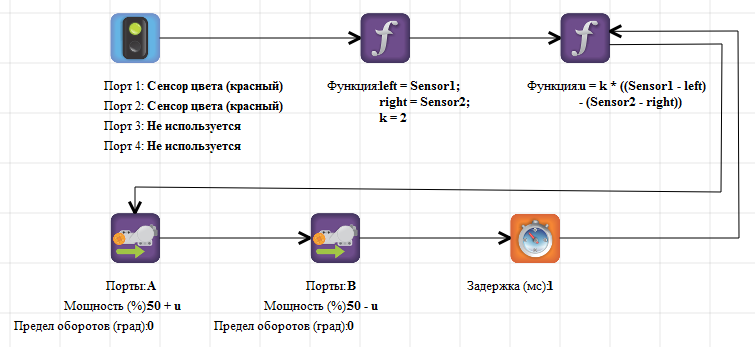
\includegraphics[width=\textwidth]{part5/5.1/alongTheLine.png}
		\caption{Движение по линии.}
		\label{image:alongTheLine}
	\end{center}
\end{figure}

Интуитивная понятность программы обеспечивается приёмом, часто используемым при проектировании 
предметно-ориентированных языков: для изображения блоков используются иконки с изображениями, 
понятными людям, видевшим робот. На блоках управления моторами нарисованы моторы Mindstorms NXT, 
блоки работы с датчиками выполнены более абстрактно, но тоже интуитивно понятны. Это 
позволяет успешно пользоваться средой даже людям, которые впервые её видят, но знакомы 
с конструктором. Кроме того, оказалось важно, что связи рисуются со стрелками на концах, 
в других средах связи стрелок не имели, и пользователи обратили на это внимание --- 
со стрелками им показалось гораздо понятнее. Это оказалось довольно неожиданным, поскольку 
направления связей всегда очевидны, и стрелки создавались исключительно как декоративные 
элементы --- для пользователей предметно-ориентированного языка может оказаться важным 
то, что кажется совершенно неважным авторам языка.

\subsection{Инструментальные средства QReal:Robots}
С помощью технологии QReal оказалось легко создать визуальный язык и редактор для него, 
однако инструментальные средства, такие как симулятор робота (далее называемый "`двухмерная модель"'), 
интерпретатор диаграмм, управляющий роботом удалённо, генератор кода для загрузки на 
робота пришлось создавать вручную. Ниже представлен краткий обзор созданных вручную 
инструментальных средств.

Наиболее объёмным по коду и сложным в реализации является интерпретатор диаграмм. 
Интерпретатор принимает на вход репозиторий с диаграммой поведения робота, и исполняет 
её, в зависимости от режима, либо на настоящем роботе посылкой ему команд по интерфейсу 
Bluetooth или USB, либо на двухмерной модели робота. Интерпретатор создавался с учётом 
следующих требований.

\begin{enumerate}
	\item Возможность исполнять программу, управляя роботом по Bluetooth или USB, в 
		зависимости от выбора пользователя.
	\item Возможность исполнять программу на двухмерной модели робота. Двухмерная модель 
		должна эмулировать окружение, способное взаимодействовать со всеми видами сенсоров 
		--- должна быть возможность задать положение стен, фиксируемых датчиками касания 
		и расстояния, и непроходимых для робота, и разноцветных линий на полу, видимых 
		для датчиков света и цвета.
	\item Архитектура интерпретатора должна позволять быстро (в течение единиц часов) 
		добавлять поддержку новых блоков визуального языка, и новых видов оборудования. 
		Должна быть возможность относительно просто и без серьёзных изменений в архитектуре 
		поддержать новые виды устройств, включая другие робототехнические конструкторы, 
		отличные от NXT, но имеющие схожую архитектуру.
\end{enumerate}

Архитектура интерпретатора представлена на рисунке~\ref{image:interpreterArchitecture}.

\begin{figure} [ht]
	\begin{center}
		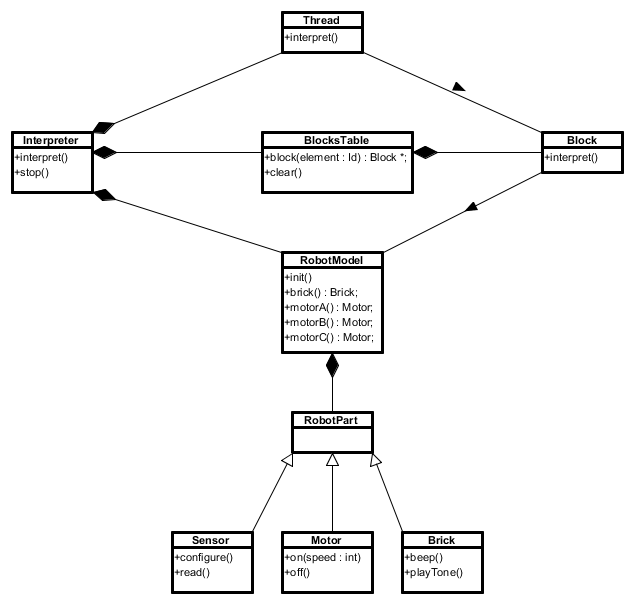
\includegraphics[width=0.9\textwidth]{part5/5.1/interpreterArchitecture.png}
		\caption{Архитектура интерпретатора.}
		\label{image:interpreterArchitecture}
	\end{center}
\end{figure}

Главный класс, который предоставляет свои функции графическому интерфейсу пользователя 
и может быть вызван из ядра системы --- Interpreter. Он содержит в себе логическую 
модель робота, таблицу блоков и список активных потоков. Логическая модель робота 
(класс RobotModel) играет роль программного интерфейса к устройству, и состоит из 
объектов (наследников RobotPart), каждый из которых реализует программный интерфейс 
к какому-либо элементу робота --- одному из датчиков, мотору, блоку управления. Эти 
объекты предоставляют высокоуровневые команды, которыми можно пользоваться при реализации 
поведения блока визуального языка, например, включение мотора, проигрывание звука. 
Таблица блоков --- это отображение блоков на диаграмме на объекты, реализующие их 
поведение. Для каждого блока языка существует свой класс (наследник Block), который 
его реализует, способный принять управление, выполнить какое-то действие (возможно, 
асинхронно), и вернуть интерпретатору следующий блок, который надо выполнить. Объекты 
этих классов создаются для каждого блока при начале работы интерпретатора и помещаются 
в таблицу, чтобы, когда управление дойдёт до какого-либо блока на диаграмме, найти 
по идентификатору блока соответствующий ему объект в таблице.

Логическая модель робота и её составные части могут быть реализованы по-разному, давая 
возможность прозрачно для реализации блоков исполнять программу на реальном роботе, 
двухмерной модели, или, потенциально, другом устройстве. Для реализации этого использован 
паттерн "`Мост"', дающий возможность для иерархии классов, видимых реализациям блоков, 
использовать заменяемые реализации. Модель робота содержит ссылку на реализацию модели 
робота, которая может быть либо логической моделью реального робота, либо логической 
моделью двухмерной модели, либо пустой моделью (модель, которая не посылает команды 
никуда, а просто эмулирует некоторое фиксированное поведение, полезна для начальной 
отладки программы). Каждый класс, представляющий датчик, имеет ссылку на реализацию, 
которая тоже может быть одного из трёх видов, аналогично самой модели. Конкретная 
модель может создавать модели датчиков своего типа, поэтому достаточно инициализировать 
интерпретатор требуемым типом модели, вся дальнейшая необходимая инициализация выполнится 
автоматически.

В случае с двухмерной моделью классы-реализации элементов модели перенаправляют запросы 
в объект класса D2RobotModel. Этот класс занимается собственно симуляцией робота, 
обсчитывая его перемещение, реакции на команды от классов-реализаций. Внешнее окружение 
моделирует отдельный класс WorldModel, и D2RobotModel может запрашивать показания 
датчика в заданной позиции и с заданным направлением у этого класса. Отображением 
результатов симуляции занимается класс D2ModelWidget. Архитектура этой части системы 
представлена на рисунке~\ref{image:twoDModelArchitecture}.

\begin{figure} [ht]
	\begin{center}
		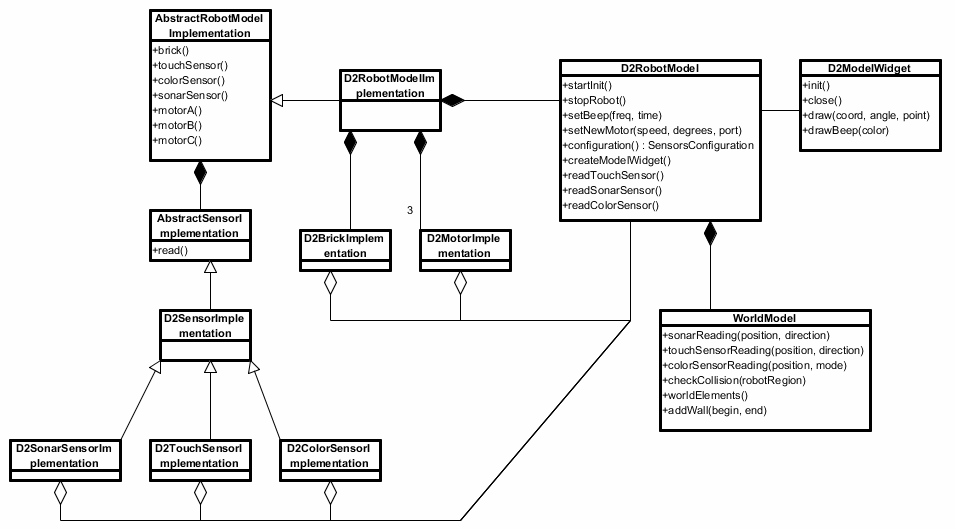
\includegraphics[width=\textwidth]{part5/5.1/twoDModelArchitecture.png}
		\caption{Архитектура двухмерной модели.}
		\label{image:twoDModelArchitecture}
	\end{center}
\end{figure}

Управление роботом по интерфейсам Bluetooth и USB использует одну логическую модель 
робота, класс RealRobotModel. Это оказалось возможно, потому что оба эти интерфейса 
используют одинаковый набор команд в примерно одинаковом формате, разнятся лишь заголовки 
пакетов с командами, передаваемых на робот. Поэтому оказалось возможным вынести транспортный 
уровень в отдельный набор классов, где инкапсулирована низкоуровневая работа с каналами 
передачи, и логическая модель просто параметризуется нужным транспортным уровнем. 
Транспорт для USB использует драйвер робота Fantom из поставки конструктора
%TODO: ссылка
, транспорт для Bluetooth работает непосредственно с системными средствами передачи 
(для работы с виртуальным COM-портом Bluetooth-канала используется сторонняя библиотека 
QextSerialPort
%TODO: ссылка
).

Окно двухмерной модели представлено на рисунке~\ref{image:twoDModelInterface}. Двухмерная 
модель моделирует одну предопределённую конфигурацию робота --- трёхколёсную тележку 
с двумя ведущими колёсами, используемую во многих задачах, связанных с движением (например, 
в робофутболе), однако можно задавать позицию и направление датчиков. Цветные линии 
на полу, видимые датчикам света и цвета, можно рисовать инструментами "`Линия"', "`Карандаш"', 
"`Эллипс"', стены --- инструментом "`Стена"'. Все элементы после размещения в рабочей 
области редактируемы, так что двухмерная модель близка по функциональности к простому 
векторному редактору. Имеется возможность сохранить нарисованную модель окружения в xml-файл.

\begin{figure} [ht]
	\begin{center}
		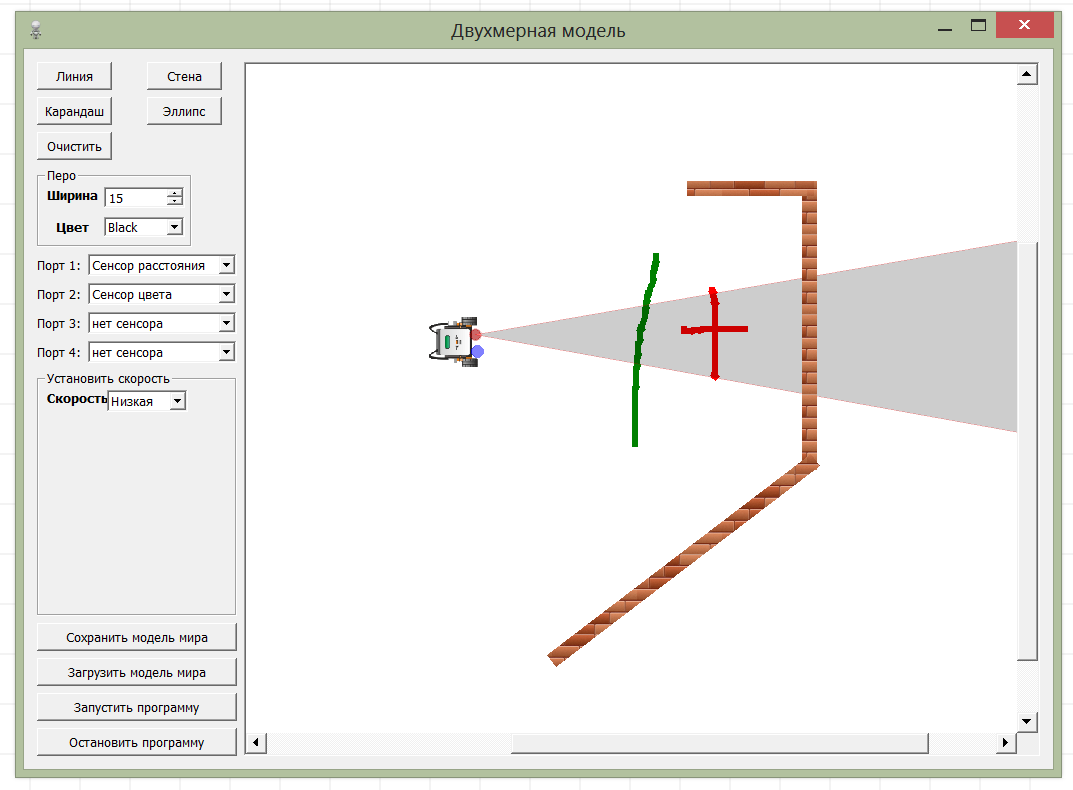
\includegraphics[width=\textwidth]{part5/5.1/twoDModelInterface.png}
		\caption{Окно двухмерной модели.}
		\label{image:twoDModelInterface}
	\end{center}
\end{figure}

Генератор кода на текстовом языке реализован в виде отдельного подключаемого модуля 
и может работать независимо от интерпретатора. Он генерирует код на языке C с использованием 
программного интерфейса операционной системы nxtOSEK
%TODO: ссылка
, на данный момент считающейся самой быстрой операционной системой для роботов Mindstorms NXT. 
Для того, чтобы сгенерированный код можно было загружать на робот, требуется, чтобы 
на роботе была установлена nxtOSEK, а на компьтере с QReal:Robots --- кросскомпилятор 
и комплект средств разработки для этой ОС. Всё необходимое для кросскомпиляции поставляется 
в виде отдельного инсталляционного пакета, который требует установленного QReal:Robots 
для установки. Решение не включать средства разработки в основной инсталляционный 
пакет QReal:Robots было принято из-за их большого объёма, что могло создать трудности 
при загрузке инсталляционного пакета пользователям, которым генерация текстовых программ 
не требуется. Генератор порождает .c-файл с кодом программы и .oil-файл с настройками 
её запуска, после чего запускается кросскомпилятор, собирающий бинарный образ программы, 
который потом загружается на робот по USB посредством утилиты из поставки конструктора. 
Для пользователя этот процесс прозрачен, ему достаточно нажать на кнопку "`Загрузить"' 
и дождаться сообщения об успешном завершении процесса загрузки. Если пользователю 
не требуется загружать программу на робот, он может просто сгенерировать код, просмотреть 
и отредактировать его во встроенном в QReal:Robots текстовом редакторе с подсветкой синтаксиса.

Генератор организован по шаблонной схеме: имеется файл с шаблоном порождаемого кода, 
в котором отмечены места, параметризуемые информацией из модели. Такие места, в свою 
очередь, могут сами заполняться текстами, сформированными с помощью шаблонов, и т.д., 
что позволяет генерировать сложно структурированные  повторяющиеся фрагменты кода. 
Пример шаблона верхнего уровня для генерации кода программы приведён ниже.

\vspace{5mm}
\begin{minipage}{\linewidth}
\begin{verbatim}
#include "kernel.h"
#include "ecrobot_interface.h"
@@BALANCER@@
@@VARIABLES@@

void ecrobot_device_initialize(void)
{
@@INITHOOKS@@
}

void ecrobot_device_terminate(void)
{
@@TERMINATEHOOKS@@
}

/* nxtOSEK hook to be invoked from an ISR in category 2 */
void user_1ms_isr_type2(void){ /* do nothing */ }

@@CODE@@
\end{verbatim}
\end{minipage}
\vspace{5mm}

С помощью текста, заключённого в "`@@"', отмечаются места для вставки параметризованного 
кода, так называемые заглушки (placeholders), генератор заменяет вхождения заглушек 
на сгенерированный для них по модели код. В приведённом выше примере заглушка @@BALANCER@@ 
заменяется на объявления функций и переменных для балансировки сегвея, если блоки 
работы с сегвеем используются на диаграмме, или пустой строкой, если таких блоков нет. 
@@VARIABLES@@ заменяется на объявления переменных --- генератор в начале работы анализирует 
все арифметические выражения в программе, формирует таблицу переменных, и все объявления 
переменных генерирует на место этой заглушки. Заглушки @@INITHOOKS@@ и @@TERMINATEHOOKS@@ 
заменяются на код инициализации и деинициализации датчиков, зависящий от того, какие 
датчики использовались в программе. 

Заглушка @@CODE@@ заменяется на код, сгенерированный по диаграмме. По каждому блоку 
визуального языка генерируется свой небольшой фрагмент программы, реализующий поведение 
этого блока. Некоторую сложность представляют конструкции, управляющие потоком исполнения 
--- условные операторы и операторы цикла. В отличие от структурных текстовых языков, 
где операторы образуют иерархическую структуру, визуальный язык позволяет связывать 
любой блок с любым блоком, что позволяет рисовать неструктурные программы, где поток 
управления попадает внутрь "`тела"' условного оператора или цикла извне. Это равносильно 
использованию оператора goto в текстовых языках, при этом визуальный язык QReal:Robots 
(как и многие другие подобные языки) не визуализирует структурные конструкции и нарушение 
структурности может произойти незаметно для программиста. Пример неструктурной программы 
приведён на рисунке~\ref{image:nonStructuredProgram}. Генератор применяет ряд эвристик 
для анализа потока исполнения программы и поиска структурных условных операторов и 
циклов. В случае, если структурный код не может быть порождён по данной диаграмме 
(как, например, представленной на рисунке), генератор выдаёт ошибку и не генерирует 
код. Такое решение было принято всвязи со спецификой применения генератора --- он 
должен порождать по возможности качественный и читаемый код, очевидным образом связанный 
с диаграммой, поскольку служит для обучения школьников программированию. Это исключает
использование goto в сгенерированном коде, и делает нежелательным использование техник goto elimination
%TODO: ссылка на оранжевую книжку про реинжиниринг
, поскольку они предполагают раскопирование неструктурных участков кода. Интерпретация 
таких диаграмм, тем не менее, вполне возможна.

\begin{figure} [ht]
	\begin{center}
		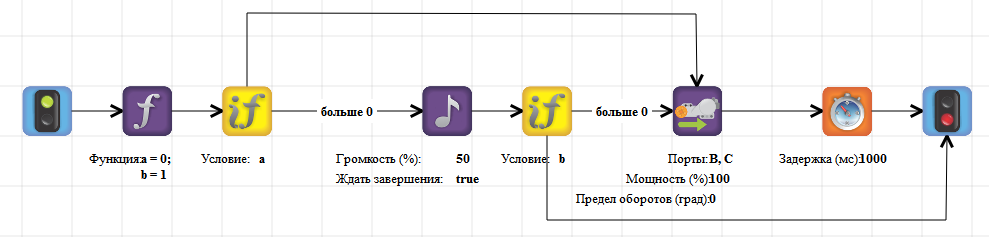
\includegraphics[width=\textwidth]{part5/5.1/nonStructuredProgram.png}
		\caption{Пример неструктурной программы.}
		\label{image:nonStructuredProgram}
	\end{center}
\end{figure}

\subsection{Опыт применения QReal}
\subsubsection{Метамодель языка QReal:Robots}
Визуальный язык QReal:Robots создавался в метаредакторе QReal. Метамодель одной из 
версий языка представлена на рисунке~\ref{image:metamodel}. Как видно, вся метамодель 
языка умещается на одном экране. Некоторая содержательная информация на рисунке не 
показана, поскольку она находится в свойствах элементов, и редактируется через редактор 
свойств (например, внешний вид элемента). Метмодель всё же слишком велика, чтобы на 
рисунке были видны все детали, поэтому ниже приводится словесное описание изображённого.

\begin{figure} [ht]
	\begin{center}
		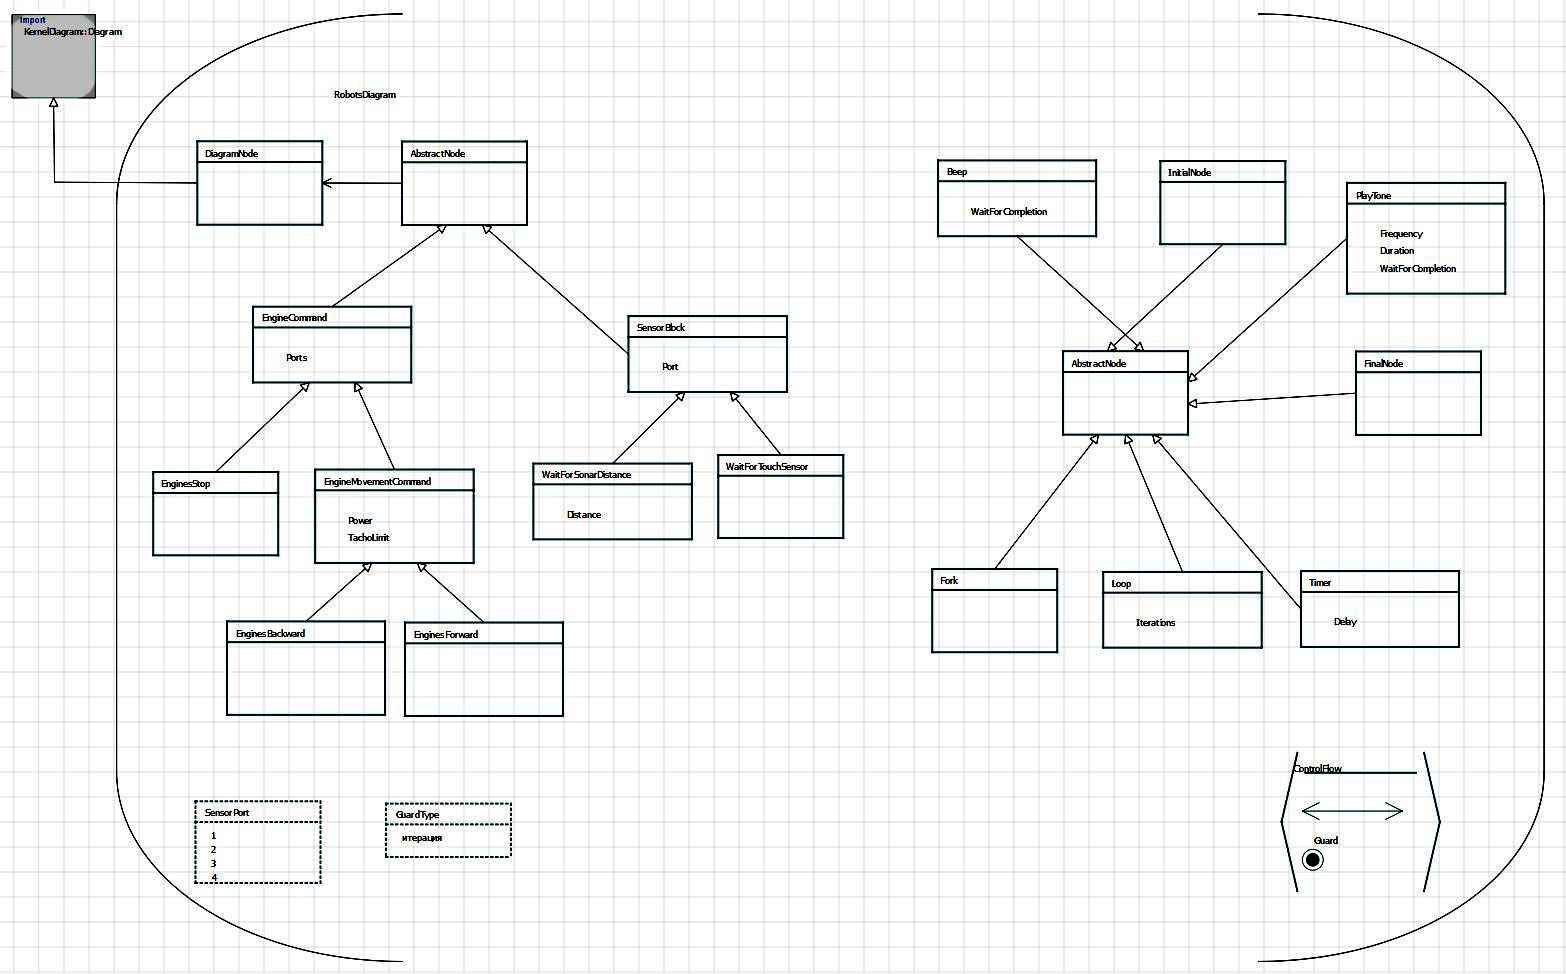
\includegraphics[width=\textwidth]{part5/5.1/metamodel.png}
		\caption{Метамодель языка QReal:Robots.}
		\label{image:metamodel}
	\end{center}
\end{figure}

Корневым элементом любой диаграммы визуального языка является узел "`Диаграмма"' 
(сущность DiagramNode в метамодели). Она наследуется от узла "`Диаграмма"', объявленного 
в импортированной метамодели KernelDiagram, получая от неё все свойства, там объявленные. 
Корнем иерархии наследования узлов языка является узел AbstractNode, который связан 
отношением Contains с DiagramNode, давая тем самым возможность всем своим наследникам 
располагаться на диаграмме. AbstractNode на рисунке~\ref{image:metamodel} имеется 
в двух экземплярах, поскольку от него наследуются все узлы языка, и отношения наследования, 
соединённые с одним AbstractNode, сделали бы диаграмму трудночитаемой --- это пример 
применения принципа разделения логической и графической моделей. Для узла AbstractNode 
не задано графическое представление, поэтому он не будет отображаться в палитре, и 
не может быть использован на диаграммах. От AbstractNode наследуется несколько конкретных 
узлов, видимых в палитре, таких как InitialNode, FinalNode (блоки "`Начало"' и "`Конец"' 
соответственно), и два абстрактных узла --- EngineCommand (блок управления двигателями) 
и SensorBlock (блок работы с датчиками). Эти узлы абстрактные, поскольку в них определяются 
свойства, общие для всех их потомков (например, порты, к которым применяются команды 
двигателей), сами они никакой смысловой нагрузки не несут и не видны в палитре. От 
EngineCommand наследуется абстактный блок EngineMovementCommand, имеющий свойство 
Power (мощность двигателя в процентах от максимальной), и конкретный блок EngineStop, 
который не требует параметра мощности, и поэтому не наследуется от EngineMovementCommand. 
Наследники EngineMovementCommand --- блоки EnginesBackward и EnginesForward, которые 
никаких своих дополнительных свойств не имеют. Кроме блоков, в метамодели описано 
одно отношение (ControlFlow, "`Поток управления"'), и два типа-перечисления: SensorPort 
(порты, к которым может быть подключен датчик), и GuardType (тип условия над связью 
"`Поток управления"', используемого в блоках "`Условие"' и "`Цикл"').

\subsubsection{Обсуждение}
Первые версии языка создавались в метаредакторе, первый прототип редактора был автоматически 
сгенерирован по метамодели в весьма короткие сроки --- всего за два-три часа, из которых 
большая часть времени ушла на поиск иконок для отображения блоков. Возможность быстро 
получить редактор языка по метамодели и удобство редактирования метамодели в метаредакторе 
позволило не только существенно сократить время разработки языка, но и дать возможность 
экспериментировать, меняя свойства и внешний вид элементов. Кроме того, метамодель 
оказалось довольно удобно сопровождать, причём не только автору языка --- работа над 
QReal:Robots в дальнейшем во многом была передана студентам, которые быстро разбирались 
в метаредакторе и могли самостоятельно добавлять в язык новые блоки или менять существующие. 
Рассматривалась даже возможность позволить самим пользователям менять свойства блоков 
языка (например, учителю скрыть ненужные в данный момент свойства блоков перед занятием), 
однако пока она не была востребована. Тем не менее, последние версии языка используют 
не графическую метамодель, а её XML-представление --- за время работы над проектом 
XML-вариант метаязыка расширился новыми возможностями, которые не были реализованы 
в графическом метаязыке, например, задание групп блоков в палитре. Несмотря на это, 
вносить изменения в язык всё же достаточно просто для людей, занимавшихся разработкой 
QReal (например, студентов).

Если технология сильно сократила время разработки визуального языка и редактора для 
него, то с созданием других средств инструментальной поддержки, таких как интерпретатора 
диаграмм или генератора кода, она смогла помочь в значительно меньшей степени. Это 
вполне ожидаемо, поскольку эти части содержат большое количество специфичных знаний 
предметной области, которые невозможно обобщить и вынести на метауровень, сделав частью 
технологии. Например, робот управляется удалённо так называемыми прямыми командами, 
которые можно посылать по интерфейсам Bluetooth или USB, и как формирование пакета 
с командой, так и логика работы с каналом передачи данных должны реализовываться вручную. 
Такого рода работы останутся трудоёмкими при любом уровне поддержки со стороны DSM-платформы, 
поскольку очень многое требуется изучить самому разработчику: систему прямых команд 
робота, API операционной системы робота для генерации кода в неё, работу с Bluetooth, 
USB, кросскомпиляцию, прошивку робота, загрузку программы на робот, и т.д. Тем не менее, 
DSM-платформа может взять на себя часть рутинной работы, и, предоставляя некий набор 
шаблонов и методологию, организовать и направить деятельность автора DSM-решения.

Наиболее интересной для автоматизации частью представляется генератор кода, поскольку 
содержит много похожего от блока к блоку кода. Генератор содержит неспецифичные для 
конкретного языка части, такие как механизм анализа потока управления, и такую низкоуровневую 
функциональность, как код формирования выходного файла или обхода модели. Некоторые 
части допускают обобщение до наиболее общей задачи генерации кода (любой генератор, 
например, должен выводить результаты в некий файл или файлы). Некоторые, такие как 
анализ потока управления, могут быть применены для всех языков, имеющих в своей основе 
семантику сетей Петри. По результатам проекта QReal:Robots было предложено два возможных 
направления автоматизации создания генераторов: вынесение общей части функциональности 
в библиотеку (или объектно-ориентированный каркас) разработки генераторов, и создание 
инструмента, который бы позволял описывать правила генерации на специализированном 
языке.  Первое направление было реализовано, библиотека поддержки разработки плагинов 
QReal теперь содержит код, общий для всех генераторов, куда вынесена функциональность 
работы с шаблонами, с выходными файлами, механизм отображения ошибок генерации. 

Была также предпринята попытка переписать генератор QReal:Robots на языке задания 
правил генерации, описанном в главе~\ref{chapter:implementation}, но она была признана 
неуспешной: оказалось, что знать ещё один текстовый язык (язык описания правил генерации) 
и работать со средством, порождающим из него генератор (в котором может быть довольно 
большое количество своих ошибок) даже менее удобно, чем писать код на языке общего 
назначения наподобие C++. Связано это ещё и с тем, что для C++ имеются хорошие среды 
разработки, тогда как на "`самодельном"' текстовом языке приходилось писать в довольно 
неудобном редакторе. В результате этого эксперимента был сделан вывод, что язык описания 
правил генерации имеет смысл попробовать сделать графическим (несмотря на то, что 
он должен активно работать с текстом), и использовать в таком случае все возможности 
самой DSM-платформы. Либо же DSM-платформа помимо создания инструментальных средств 
для визуальных языков должна позволять создавать удобные инструментальные средства 
и для текстовых языков, чтобы предметно-ориентированные текстовые языки могли эффективно 
применяться как в DSM-решениях, так и для нужд самой DSM-платформы так же, как применяются 
сейчас визуальные языки. Оба эти направления приводятся здесь, как возможности для 
дальнейшего исследования, и выходят за рамки данной работы --- в QReal как на момент 
создания DSM-решения QReal:Robots, так и на момент написания этой диссертации для 
написания генераторов используется язык C++.

Вторая возможная цель автоматизации создания дополнительных инструментальных средств 
для языка --- интерпретатор диаграмм. В QReal:Robots интерпретатор был написан целиком 
на C++, и, как и в случае с генератором,  усилия на его разработку удалось бы значительно 
сэкономить, если бы существовала библиотека (или каркас) с общим для всех интерпретаторов 
кодом. Сам процесс интерпретации как последовательности передачи токенов исполнения и 
выполнения некий действий в узле, получившем токен, общий для всех языков с семантикой, 
основанной на сетях Петри, поэтому может быть реализован языконезависимым образом. 
Действия, выполняемые в узлах, сильно языкозависимы (не все, блоки ветвления, параллельного 
исполнения, начала и конца программы могут присутствовать во многих языках и иметь 
одинаковую семантику). Специфичные для конкретного языка действия можно реализовывать 
на языке общего назначения, либо же на каком-либо интерпретируемом языке общего назначения, 
наподобие Python
%TODO: ссылка
или F\#
%TODO: ссылка
. Использование интерпретируемых языков имеет весомое преимущество --- действия можно 
модифицировать без пересборки интерпретатора, это могут делать в том числе и сами 
пользователи DSM-решения. Недостаток такого подхода очевиден: на всех машинах, где 
используется DSM-решение, требуется наличие интерпретатора выбранного языка. Поскольку 
на данный момент задача интерпретации достаточно сложных диаграмм возникала только 
в QReal:Robots, задача автоматизации создания интерпретаторов в рамках проекта QReal 
серьёзно не рассматривалась, и соображения выше приведены здесь как возможные направления 
дальнейшей работы.

\subsection{Результаты проекта QReal:Robots}
Проект QReal:Robots, по мнению автора, полностью доказал состоятельность предметно-ориентированного 
подхода и работоспособность подходов, реализованных в проекте QReal и описываемых в 
данной работе. В результате проекта с помощью DSM-платформы была создана система визуального 
программирования, которая оказалась не хуже разработанных вручную, при этом время 
на разработку визуального редактора для этой системы удалось с помощью DSM-платформы 
сократить в несколько десятков раз по сравнению с разработкой редактора с такой же 
функциональностью вручную. Однако выигрыш во времени при разработке и доведении до 
отчуждаемого продукта всей системы в целом оказался не таким значительным, как при 
разработке визуального редактора --- многие задачи оказались неавтоматизируемы в принципе. 
В ходе проекта были выявлены задачи, решение которых позволило бы уменьшить трудоёмкость 
создания подобных систем. В целом DSM-подход показал себя полезным на практике, и 
дальнейшие исследования в этой области помогли бы эффективно создавать специализированные 
среды визуального программирования и для гораздо более узких предметных областей.

Результат проекта --- среда QReal:Robots --- была представлена на "`Открытых состязаниях 
Санкт-Петербурга по робототехнике"' 2012 года и на робототехническом фестивале "`Робофест 2012"' 
в Москве. В качестве доказательства применимости этой среды к реальным задачам, решаемым 
школьниками с помощью сред-аналогов, команда студентов приняла участие в соревнованиях 
в движении робота по линии с программой, реализованной на QReal:Robots. Несмотря на 
то, что для студентов кафедры системного программирования участие в соревнованиях 
стало практически первым опытом решения задач кибернетики, им удалось показать достойные 
результаты, уступив фактически лишь специально созданным для этой задачи роботам (которые 
по техническим характеристикам имели преимущество перед роботами, собранными из конструктора 
Mindstorms NXT). На соревнованиях было проведено анкетирование школьников, которым 
было предложено решить некоторые простые задачи на QReal:Robots, результаты показали, 
что пользовательский интерфейс продукта достаточно хорош, чтобы вызвать у пользователей 
симпатию
%TODO: (подробнее об исследовании пользовательского интерфейса QReal:Robots см. в работе [ссылка на доклад на списке Соковиковой])
. С использованием QReal:Robots было также проведено занятие в детском робототехническом 
лагере в г. Сиверский летом 2012 года, где школьники успешно решили задачу движения 
робота по линии на двухмерной модели.

Кроме соревнований, среда QReal:Robots представлялась на стендовых докладах при соревнованиях, 
и на нескольких специализированных конференциях школьных учителей и методистов 
%TODO (названия конференций и ссылки на опубликованные тезисы (мои тезисы с конференции в Петербурге не опубликовали, так что надо название конференции привести))
, где вызвала большой интерес среди учителей. Некоторые из них впоследствии обращались 
к автору с предложением оказать посильную помощь в разработке и тестировании, некоторые 
использовали QReal:Robots в своих занятиях. Таким образом, QReal:Robots можно считать 
полноценным отчуждаемым продуктом, востребованным и имеющим реальных пользователей, 
в том числе и не владеющих программированием.
